%%%%% Please set the path to 'beamer' directory in your environment %%%%%
\newcommand{\beamerDir}[0]{/mnt/c/Users/atsushi/Documents/workspace/env/Beamer/beamer/beamer/}


%%%%% Load setting %%%%%
\documentclass[aspectratio=169, dvipdfmx, 12pt, compress]{beamer}% dvipdfmxしたい

%%%%% Packages %%%%%
\usepackage{bxdpx-beamer}% dvipdfmxなので必要
\usepackage{pxjahyper}% 日本語で'しおり'したい
\usepackage{tikz}
\usepackage{tcolorbox}
\usetikzlibrary{shapes}
\usepackage{xcolor}
\usepackage[absolute,overlay]{textpos}
\usepackage{adjustbox}
\usepackage{caption}
\usepackage{ifthen}


%%%%% Settings %%%%%
\usetheme[sectionpage=progressbar, subsectionpage=progressbar]{metropolis}
% block style
\metroset{block=fill}
% space between line
\renewcommand{\baselinestretch}{1.3}
% space between item
\newlength{\wideitemsep}
\setlength{\wideitemsep}{0.9\itemsep}
% \addtolength{\wideitemsep}{1.0pt} <- more space
\let\olditem\item
\renewcommand{\item}{\setlength{\itemsep}{\wideitemsep}\olditem}
% frame title
\definecolor{coolblack}{rgb}{0.0, 0.18, 0.39}
\setbeamercolor{frametitle}{bg=coolblack!90,fg=white}
\setbeamerfont{frametitle}{size=\large}
\addtobeamertemplate{frametitle}{}{\vspace{-1em}}
\makeatletter
\setlength{\metropolis@frametitle@padding}{1.4ex}% <- default 2.2 ex
% foot line
\addtobeamertemplate{footline}{}{\vspace{-1em}}
% normal text color
\setbeamercolor{normal text}{fg=black!80}
% progress bar
\definecolor{lightgray}{rgb}{0.83, 0.83, 0.83}
\setbeamercolor{progress bar}{bg=lightgray, fg=coolblack}
\setbeamersize{text margin left=15pt, text margin right=15pt}
% equation font
\usefonttheme{professionalfonts}
% Change standard block width
\addtobeamertemplate{block begin}{%
    \centering
    \begin{columns}\begin{column}{0.9\textwidth}
            \centering
            }{}
            \addtobeamertemplate{block end}{}{\end{column}\end{columns}}
% Change alert block width
\addtobeamertemplate{block alerted begin}{%
    \centering
    \begin{columns}\begin{column}{0.9\textwidth}
            \centering
            }{}
            \addtobeamertemplate{block alerted end}{}{\end{column}\end{columns}}
% Change example block width
\addtobeamertemplate{block example begin}{%
    \centering
    \begin{columns}\begin{column}{0.9\textwidth}
            \centering
            }{}
            \addtobeamertemplate{block example end}{}{\end{column}\end{columns}}
% Itemize color
\setbeamertemplate{itemize item}{\color{black}\scriptsize$\blacksquare$}
\setbeamertemplate{itemize subitem}{\color{black}\scriptsize$-$}
% Simplification  color
\definecolor{cobalt}{rgb}{0.0, 0.28, 0.67}
\setbeamercolor{block title example}{fg=black!80,bg=cobalt!35}
\setbeamercolor{block body example}{fg=black,bg=cobalt!15}
% Definition
\BeforeBeginEnvironment{definition}{
    \setbeamercolor{block title}{use=alerted text, bg=alerted text.fg!70,fg=white}
    \setbeamercolor{block body}{use=alerted text, bg=alerted text.fg!20}
}
\AfterEndEnvironment{definition}{% return to default
    \setbeamercolor{block title}{use=structure,fg=structure.fg,bg=structure.fg!20!bg}
    \setbeamercolor{block body}{parent=normal text,use=block title,bg=block title.bg!50!bg, fg=black}
}
% Theorem
\definecolor{seagreen}{rgb}{0.18, 0.55, 0.34}
\setbeamertemplate{theorems}[numbered]
\BeforeBeginEnvironment{theorem}{
    \setbeamercolor{block title}{fg=black!80,bg=seagreen!40}
    \setbeamercolor{block body}{fg=black,bg=seagreen!15}
}
\AfterEndEnvironment{theorem}{% return to default
    \setbeamercolor{block title}{use=structure,fg=structure.fg,bg=structure.fg!20!bg}
    \setbeamercolor{block body}{parent=normal text,use=block title,bg=block title.bg!50!bg, fg=black}
}
% Lemma
\undef{\lemma}
\newtheorem{lemma}{\translate{Lemma}}
\BeforeBeginEnvironment{lemma}{
    \setbeamercolor{block title}{fg=black!80,bg=seagreen!20}
    \setbeamercolor{block body}{fg=black,bg=seagreen!10}
}
\AfterEndEnvironment{lemma}{% return to default
    \setbeamercolor{block title}{use=structure,fg=structure.fg!80,bg=structure.fg!20!bg}
    \setbeamercolor{block body}{parent=normal text,use=block title,bg=block title.bg!50!bg, fg=black}
}


%%%%% Original Command %%%%%
\newcommand{\subt}[1]{\vspace{-2mm}{\fontsize{10pt}{0cm}\selectfont \textcolor{lightgray}{#1}}\vspace{-1mm}}
\newcommand{\lastpage}[0]{\begin{frame}\begin{textblock*}{1.0\linewidth}(0pt, 50pt)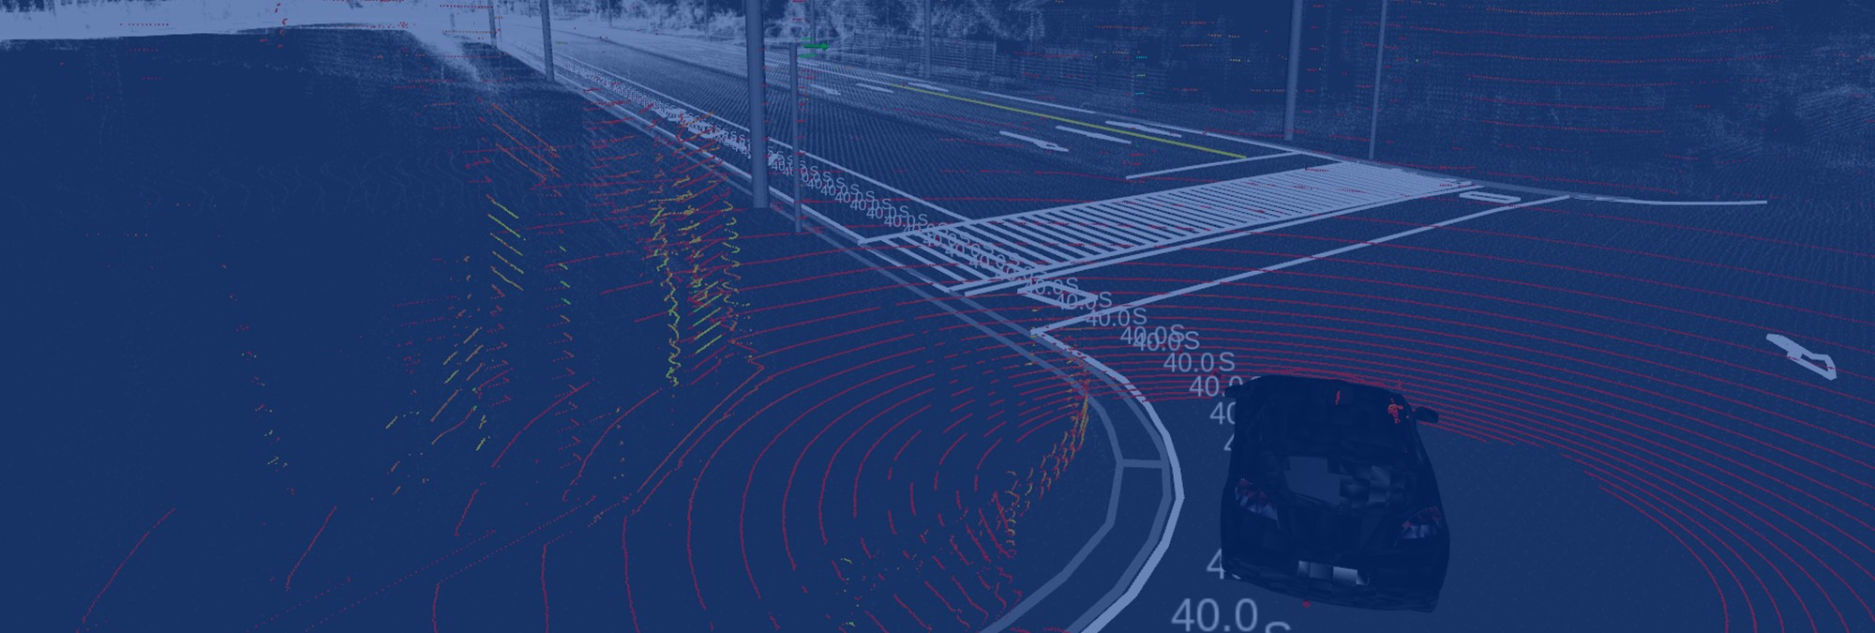
\includegraphics[scale=0.512]{\beamerDir/master_figure/last.pdf}\end{textblock*}\end{frame}}
\newcommand{\todo}[1]{\al{\LARGE\textbf{TODO:} #1}}
\newcommand{\headerheight}[0]{5mm}
\newcommand{\footerheight}[0]{5mm}
\newcommand{\slideheight}[0]{\textheight-\headerheight-\footerheight}
\newcommand{\tabml}[1]{\hspace{-2.1mm}\begin{tabular}{l} #1 \end{tabular}}
\newcommand{\al}[1]{\alert{#1}}
\newcommand{\argempty}[0]{}
\newcommand{\onlyslide}[1]{
    \vspace{\headerheight}
    \begin{minipage}[c][\slideheight][c]{\textwidth}
        #1
    \end{minipage}
}
\newcommand{\onlyimage}[1]{
    \onlyslide{
        \centering
        \begin{columns}
            \begin{column}{\textwidth}
                \centering
                \adjustbox{max width=\textwidth, max height=\slideheight}{
                    \includegraphics{#1}
                }
            \end{column}
        \end{columns}
    }
}
% fit image
\newlength\fitimageht
\newlength\fitotherht
\newsavebox\fitimagebox
\newcommand{\fitimage}[2]{%
    \sbox\fitimagebox{%
        \parbox{\textwidth}{%
            #1\par
        }%
    }%
    \settototalheight{\fitotherht}{%
        \usebox\fitimagebox
    }%
    \setlength\fitimageht{\textheight}%
    \addtolength\fitimageht{-\fitotherht-\headerheight-\footerheight-1\baselineskip}%
    \vspace{\headerheight}
    #1\par
    \centering
    \includegraphics[width=\textwidth,height=\fitimageht,keepaspectratio]{#2}
}
% Simplification
\newcommand{\assume}[1]{
    \begin{exampleblock}{Simplification }
        #1
    \end{exampleblock}
}
% Re-post
\setbeamercolor{RepostBox}{fg=black!50, bg=coolblack!10}
\newcommand{\repost}[1]{
    \vspace{2mm}
    \centering
    \begin{columns}
        \begin{column}{0.86\textwidth}
            \begin{beamercolorbox}[wd=\textwidth, sep=2pt, rounded=true, shadow=true]{RepostBox}
                \begin{tabular}{|p{0.95\textwidth}}
                    {\fontsize{10pt}{10pt}#1}
                \end{tabular}
            \end{beamercolorbox}
        \end{column}
    \end{columns}
}

% equation ballon
\tcbset{
    framebox/.style={
            enhanced,
            boxsep=0pt,       % 箱の上下左右の余白を指定
            colback=white,
            boxrule=1pt,
            colframe=#1
        },
    framebox/.default=red
}
\newcommand{\upbln}[3]{
    \tcboxmath[
        framebox=#2,
        top=0.5ex,bottom=0.5ex,    % 箱の上下の余白を指定
        left=0.5ex,right=0.5ex,    % 箱の左右の余白を指定
        overlay={
                \node[
                    above,
                    rectangle callout,                         % nodeを吹き出しの形に
                    callout absolute pointer={(frame.north)},  % 吹き出しの先端を絶対的に指定
                    fill=#2!20
                ] at ([yshift=2ex]frame.north) {\footnotesize#3};
            }
    ]{#1}
}
\newcommand{\lwbln}[3]{
    \tcboxmath[
        framebox=#2,
        top=0.5ex,bottom=0.5ex,    % 箱の上下の余白を指定
        left=0.5ex,right=0.5ex,    % 箱の左右の余白を指定
        overlay={
                \node[
                    below,
                    rectangle callout,                         % nodeを吹き出しの形に
                    callout absolute pointer={(frame.south)},  % 吹き出しの先端を絶対的に指定
                    fill=#2!20
                ] at ([yshift=-2ex]frame.south) {\footnotesize#3};
            }
    ]{#1}
}
\tcbuselibrary{theorems,skins}



%%%%% Mode %%%%%
% \newcommand{\forme}[1]{#1}
\newcommand{\forme}[1]{}


%%%%% Front Cover %%%%%
\title{Automatic Latency Management for ROS2 Benefits Challenges and Open Problems}
\subtitle{IEEE Real-Time and Embedded Technology and Applications Symposium (RTAS), 2021}
\author{矢野 篤志}
\date{\today}
\institute[EMBIV]{EMBIV}
\logo{\begin{textblock*}{0.1\linewidth}(2pt, 237pt)
\includegraphics[scale=0.4]{\beamerDir/master_figure/Emb_logo.pdf}\end{textblock*}}


%%%%% Document Start %%%%%
\begin{document}

\maketitle

% \summary{0}{0}
% % !TeX root = main.tex


\begin{frame}{提案の概要}
    \begin{itemize}
        \item 優先度駆動型スケジューリングによってROSのリアルタイム性能と予測可能性を大幅に改善できることを主張する
        \item 主張を裏付けるために, 優先度駆動型チェーン考慮スケジューリングに関する我々の研究をレビューし, Apex.AI が開発したオープンソースリファレンスシステムを用いた評価を行う
        \item ROS 2のリアルタイム性能を向上させるために不可欠な以下2つの課題を説明する
        \begin{itemize}
            \item マルチスレッドエグゼキュータ設計
            \item アクセラレータサポート
        \end{itemize}
    \end{itemize}
\end{frame}


\begin{frame}{Outline}
    \setbeamertemplate{section in toc}[sections numbered]
    \scriptsize\tableofcontents[hideallsubsections]
\end{frame}

% !TeX root = main.tex

\section{PRIOR KNOWLEDGE}
\label{sec: prior knowledge}

\begin{frame}{前提知識}
    \begin{itemize}
        \item \ourl{ROS}{https://tier4.atlassian.net/wiki/spaces/EMBIV/pages/2683603071/ROS+Robot+Operating+System}
        \item \ourl{publish/subscribeモデル}{https://tier4.atlassian.net/wiki/spaces/EMBIV/pages/2675048610/Publish+Subscribe}
        \item \ourl{SCHED\_DEADLINE}{https://tier4.atlassian.net/wiki/spaces/EMBIV/pages/2692645566/SCHED+DEADLINE}
        \item \ourl{最大イベント到着曲線}{https://drive.google.com/file/d/1n85X0vDrDm4IDANDP4aUoC0SNnZLAiRN/view?usp=share_link}
        \item \ourl{Casiniらによる先行研究}{https://drive.google.com/file/d/1sHujFqbmgCoJbC6g6KdC7ihua4Jqddju/view?usp=share_link}
    \end{itemize}
\end{frame}

% !TeX root = main.tex

\section{INTRODUCTION}
\label{sec: introduction}

\begin{frame}{}
    \begin{itemize}
        \item ロボット工学のような, 様々な分野の深い専門知識を必要とする学際的で複雑なアプリケーション領域では, 通常, 全ての, あるいはほとんどのソフトウェアをゼロから書くという選択肢はあり得ない
        \item その代わりに, ロボット工学者は, ROSのような一般的なロボット工学フレームワークで容易に利用できる, 標準機能を提供する既存のサードパーティコンポーネントの統合を採用するのが一般的である
        \item その利点は数多く, 簡単に理解できる
        \item 例えば, 複数の最新パス計画アルゴリズムと3D可視化サポートを備えた完全なナビゲーションスタックがたった1回のダウンロードで手に入るなら, なぜ新しいナビゲーションサブシステムを苦労して開発する必要があるか?
    \end{itemize}
\end{frame}

\begin{frame}{}
    \begin{itemize}
        \item 完全なロボットシステムを構築するためには, 多くの相互作用するコンポーネントを統合する必要がある
        \item ROS開発プロセスの分散型オープンソースの性質により, これらのコンポーネントは通常, 必ずしもお互いを知らない複数の独立したコンポーネント開発者によって分離して開発される
        \item 同様に, システムインテグレータは, アプリケーションおよびミッション固有のロジックと「グルーコード」で展開プラットフォーム上で選択したコンポーネントを構成するが, 通常, それぞれのコンポーネント開発者と密接に連携することはない
    \end{itemize}
\end{frame}

\begin{frame}{}
    \begin{itemize}
        \item コンポーネントの統合を可能な限りシンプルに保つために, ROSはコンポーネントの疎結合を可能にする古典的なトピックベースのpublish/subscribeパラダイムを採用している
        \item 概念的には, 各コンポーネントは, 特定のトピックをsubscribeする多数のコールバックを含む「ブラックボックス」として理解できる
        \item 与えられたトピックに関連するメッセージがpublishされるたびに, 全てのsubscribeコールバックが呼び出され, 何らかの計算を実行し, 次に他のトピックに後続のメッセージをpublishすることができ, これがさらにコールバックをトリガするというように, 繰り返す
    \end{itemize}
\end{frame}

\begin{frame}{}
    \begin{itemize}
        \item インテグレータは, あるコンポーネントの「入力コールバック」を別のコンポーネントの「出力トピック」に接続することによってコンポーネントを構成する
        \item ROSシステムは, このように相互接続されたトピックとコールバックの複雑なネットワークを形成し, データ (環境刺激など) は, イベント駆動型の方法でネットワークを通じてcause-effectチェーンに沿って伝播し, インテグレータが望むように透過的にコンポーネント境界を交差させることができる
    \end{itemize}
\end{frame}

\begin{frame}{}
    \begin{itemize}
        \item このようなcause-effectチェーンの典型的な例として, 進路上の障害物を検知して反応する必要のある移動ロボットのセンシング-計算-行動パイプラインが挙げられる
        \item 例えば, ハードウェアドライバコンポーネントがレーザースキャナから新しいサンプルを取得し (cause) , それが複数のマッピング, 座標変換, パス計画, 車輪制御コンポーネントを経て, 最終的に車輪速度の変化 (effect) をもたらす可能性がある
        \item このようなデータ処理のチェーンにおいて, causeからeffectまでの最大レイテンシ時間は, ロボットが正しく機能するために重要な役割を果たすことは明らかであり, また, 安全性を考慮する上でも重要であることが多い
    \end{itemize}
\end{frame}

\begin{frame}{}
    \begin{itemize}
        \item 重要なのは, システムインテグレータにできるだけ多くの展開の選択肢を残し, コンポーネントの再利用の機会を最大化するために, ROSの実行管理層と基礎となるオペレーティングシステムは, 意図的にコンポーネント開発者に公開されないことである
        \item むしろ, ROSの中心的なコールバック抽象化は, コールバック手続きがいつどのようにスケジュールされるか, コールバックの実行がスレッドまたはプロセスにわたってどのように組織されるか, またはネットワーキング層がメッセージの送受信をどのように処理するかを全く意識せずに, 実行から完了までセマンティクスを持つ単なる手続きである
    \end{itemize}
\end{frame}

\begin{frame}{}
    \begin{itemize}
        \item ROSはオープンソースソフトウェアであるため, 原理的にはシステムの実行と通信の挙動を完全に理解し制御することが可能である
        \item このため, リアルタイムシステムの専門家から見れば, ROSにリアルタイムシステム研究でよく知られた技術を導入することは論理的なステップであるように思える可能性がある
        \item しかし, 一見したところ, これを難しくしているハードルがいくつかある
    \end{itemize}
\end{frame}

\begin{frame}{}
    \begin{itemize}
        \item まず第一に, インテグレータに必要な情報が不足している
        \item ほとんどのリアルタイム分析では, 同時実行タスクの数, それらの起動セマンティクスや機能的相互作用, メッセージの到着パターン, 最悪実行時間など, 多くの低レベルシステムの詳細に関する深い知識が前提となっている
        \item ROSコンポーネントは, この種の情報を提供するマニフェストと一緒に来ることはない
        \item さらに悪いことに, リアルタイム分析は, 欠陥のある情報や不完全な情報にうまく対処できない
        \item モデリング目的でサードパーティコンポーネントを手作業でリバースエンジニアリングしているときに, たった一つのミスや見落としがあれば, その取り組み全体を無条件に無効にしてしまうことになりかねない
    \end{itemize}
\end{frame}

\begin{frame}{}
    \begin{itemize}
        \item 第二に, 必要なシステムの詳細をコンポーネントレベルで静的に決定し, 記述することができない
        \item その理由のひとつは, 多くのロボット工学アルゴリズムが, ユースケースやプラットフォーム固有の側面に依存し, 実行時間や起動パターンが大きく変化するためである
        \item 例えば, ビデオストリーム中の物体を識別し, その軌跡を推測する一般的な物体追跡コンポーネントを考えてみよう (例えば, 隣の車線の車など)
        \item この機能の実行時間は, ビデオストリームのフレームレート, 解像度, コーデック, および特定のトラッキングアルゴリズムに関連する他の様々なパラメータを含む, 様々なパラメータに依存する
        \item これらのパラメータは, 一般的なオブジェクトトラッキングコンポーネントの開発者が前もって知っていたり, 固定されていたりするものではない
    \end{itemize}
\end{frame}

\begin{frame}{}
    \begin{itemize}
        \item このようなユースケース特有の情報は, 特定のロボットを構築するインテグレーターにしか分からない
        \item インテグレーターは, 必ずしもオブジェクトトラッキングやリアルタイムシステムの専門家ではないため, 特定の構成を選択した場合の影響を常に予測できるわけではない
        \item したがって, コンポーネントのリソース要求とリアルタイム動作は, 常に特定の展開で使用するという文脈で評価されなければならない
        \item これは, ROSフレームワークの人気の根底にある「ブラックボックス」コンポーネントのモジュール式再利用と相容れるものではない
    \end{itemize}
\end{frame}

\begin{frame}{}
    \begin{itemize}
        \item 最後に, 仮にインテグレータが各コンポーネントについてそれぞれの専門家と議論し, タイミング分析に必要な全ての詳細を入手できたとしても, 第三の根本的な問題が残る
        \item 多くのコンポーネントのリソース要件と性能特性は, 本質的にロボットの動的環境に依存し, したがって時間とともに変化するため, 静的 (最悪のケース) リソース配置は実行不可能なのである
    \end{itemize}
\end{frame}

\begin{frame}{}
    \begin{itemize}
        \item 例えば, 前述の物体追跡コンポーネントと, ランドマークベースの自己位置特定コンポーネントに依存するロボットを再度考えてみよう
        \item 一方, 人口が少ない田舎町よりも, にぎやかな街中を移動する方が, 物体追跡装置の処理時間はずっと長くなる
        \item 一方, 認識可能なランドマークが多い都市部では, ほぼ一様な風景よりも自己位置推定がはるかに容易である可能性が高い
        \item どちらの状況でも十分なリソースを確保するためには, システムインテグレーターは, 不毛の土地からなる賑やかな都市を想定したシステムを用意しなければならない
    \end{itemize}
\end{frame}

\begin{frame}{}
    \begin{itemize}
        \item ロボット工学では, このような悲観的なシステム設計を行うと, すぐに現実的な限界に直面することになる
        \item その代わりに, 実用的で費用対効果の高いシステムを維持するためには, 各コンポーネントのピーク需要の合計ではなく, 予想されるジョイントリソースのピーク需要に対してプロビジョニングを行う必要がある
    \end{itemize}
\end{frame}

\begin{frame}{貢献する}
    \begin{itemize}
        \item これらの課題を克服するために, 我々は, 実行時に動的にタイミングを考慮した方法でROSシステムをプロビジョニングするための自動レイテンシマネージャを使用することを提案する
        \item 具体的には, ROS Live latency manager (ROSLlama) を紹介する
        \item これは, 重要なcause-effectチェーンに沿ったレイテンシを, 非リアルタイム専門家が使いやすく, かつ設定にあまり手間をかけない方法で, 既存のリアルタイム機構を使用して制御することを可能にする
    \end{itemize}
\end{frame}

\begin{frame}{貢献する}
    \begin{itemize}
        \item ROS-Llamaは, 複雑なシステムパラメータをユーザに要求するのではなく, 実行時に必要なパラメータを自動的に推定し, 状況の変化に応じてスケジューリングパラメータを動的に調整することが可能である
        \item もし, 指定されたレイテンシの目標が全て同時に達成できない場合 (例えば, 不利な環境条件による一時的な過負荷が原因) , ROS-Llamaは制御された緩やかなデグレードプロセスを開始し, システムインテグレーターが純粋に宣言的な方法で (すなわち, cause-effectチェーンがどの部品を通過しているかを理解しなくても) cause-effectチェーンの重要性を特定できるようにする
    \end{itemize}
\end{frame}

\begin{frame}{本論文の貢献}
    \begin{itemize}
        \item  ロボティクス領域における動的レイテンシ管理問題を探求し, 実用的なソリューションが満たさなければならない制約と要件を文書化する (第III章)

        \item  ROSのための最初の自動レイテンシマネージャであるROS-Llamaの設計と実装を紹介する (セクションIV)

        \item 標準的な Linux システム上の ROS コンポーネントを用いて, ROS-Llama が移動ロボットのcause-effectチェーンのレイテンシをうまく制御できることを示す評価について報告する (セクションVI)

    \end{itemize}
\end{frame}

\begin{frame}{}
    \begin{itemize}
        \item ROS-Llamaは, 数年にわたる研究とエンジニアリングの努力の結果であり, その間, 我々は多くの課題や技術的な限界に遭遇した
        \item セクションVIIでは, 以下の点を強調する
              \begin{itemize}
                  \item  ROS-Llamaをより効果的かつ正確にするための分析改善の機会
                  \item  ROSとLinuxのプラットフォームには, システムのさらなる改良の妨げとなる大きな限界がある
              \end{itemize}
    \end{itemize}
\end{frame}

% !TeX root = main.tex

\section{BACKGROUND AND DEFINITIONS}
\label{sec: background and definitions}

\begin{frame}{セクションサマリ}
    \begin{itembox}[l]{\textbf{目的}}
        必要な背景知識と ROS-Llama の基礎となる主要な分析概念を簡単にまとめます
    \end{itembox}
\end{frame}

\begin{frame}{ROS}
    \begin{itemize}
        \item ROS フレームワークは, ロボット工学アプリケーション向けの人気のあるオープンソースミドルウェアおよびコンポーネントリポジトリである [1]
        \item 本論文は特に, 第一世代のROSフレームワークの最近の主要なリファクタリングであるROS 2 [2]に関連している
        \item 簡潔にするために, 本論文ではバージョン番号を省略する
    \end{itemize}
\end{frame}

\begin{frame}{}
    \begin{itemize}
        \item ROS は, 通常 Linux に展開される成熟した機能豊富なミドルウェアである
        \item レイテンシ管理に不可欠な重要なランタイム要素であるトピック, コールバック, エグゼキュータに焦点を当てている
    \end{itemize}
\end{frame}

\begin{frame}{}
    \begin{itemize}
        \item すでに述べたように, ROS は, 展開の選択をほとんど意識しない publish/subscribe インフラストラクチャを中心に構築されている
        \item したがって, ROS アプリケーションは, 複数のホスト, コア, プロセス, およびスレッドにまたがることができる
        \item 自動レイテンシ管理の目的では, Linux を実行する共有メモリマルチコアシステムが自然な範囲であり, 我々はここに注意を限定する
    \end{itemize}
\end{frame}

\begin{frame}{}
    \begin{itemize}
        \item 概念レベルでのトピックとコールバックについては, セクションI で既に説明した
        \item 実装レベルでは, ROS アプリケーションは 1 つまたは複数のプロセスで構成され, 各プロセスは 1 つまたは複数のスレッドで構成され, 次にエグゼキュータ (すなわち, コールバックを呼び出す ROS ライブラリ機能) を実行する
        \item 各コールバックは, 特定のエグゼキュータに関連付けられている
        \item 新しいメッセージがトピックに投稿されると, ROS ミドルウェアは, トピックのsubscriberにサービスを提供するエグゼキュータをホストする全てのスレッドに, メッセージのコピーが確実に配信されるようにする
        \item 標準的な構成では, ROSはエグゼキュータ間でメッセージを仲介するためにDDSミドルウェアに依存しており, 適切なDDS実装が複数存在する[3-5]
    \end{itemize}
\end{frame}

\begin{frame}{}
    \begin{itemize}
        \item 新しいメッセージが利用可能であることがエグゼキュータに通知されると, 対応するコールバックがアクティブになり, 実行のためにキューに入れられる
        \item したがって, コールバックがメッセージを処理するレイテンシは, 2つの主要な要因によって決定される (i) OSがそれぞれのエグゼキュータをホストするスレッドに割り当てるプロセッサ時間, および (ii) エグゼキュータが保留中のコールバックの起動をどのようにシーケンスするかによって発生する待ち行列のレイテンシ
    \end{itemize}
\end{frame}

\begin{frame}{}
    \begin{itemize}
        \item 本論文の目的では, 側面 (i) のエグゼキュータスレッドのスケジューリングが主な関心事である
        \item これは, 自動レイテンシマネージャーが実行時に制御できる主な要因であるためである
        \item 側面 (ii) の待ち行列のレイテンシも, コールバックのレイテンシに大きな影響を与え, 分析するのは決して簡単ではない [6] が, (現在の ROS バージョンでは) ランタイム管理には適していない
    \end{itemize}
\end{frame}

\begin{frame}{応答時間分析}
    \begin{itemize}
        \item 我々は, (ii), すなわち, ROSのデフォルトのエグゼキュータによって管理されるコールバックの応答時間を制限するために, Casiniらによる先行研究[6]に依存している
        \item Casini らは, ROS システムを, アクティベーション関係によって接続されたコールバックの有向 非循環グラフ (DAG) としてモデル化し, 処理チェーン, すなわちコールバック DAG の任意のパスのエンドツーエンドレイテンシ境界について, 実行者を意識した最悪応答時間を提供しています
        \begin{itemize}
            \item 実際には, ROSアプリケーションは常に非周期的であるとは限らない
            \item ROS-Llamaが抽出されたコールバックグラフのサイクルを回避する方法については, Sec.Vで説明する
        \end{itemize}
    \end{itemize}
\end{frame}

\begin{frame}{予約}
    \begin{itemize}
        \item Casiniらは各スレッドの供給境界関数 (SBF) [7] が既知であるという仮定の下で, 最悪応答時間を提供する
        \item SBFはあるスレッドがOSのスケジューラから与えられた区間にどれだけの処理時間を割り当てられることが保証されているかを特徴づける
        \item これにより, スケジューリング分析では, 長さ $\Delta$ の任意の間隔で $s b f(\Delta)$ 単位の処理時間を提供する分離されたコアで実行されているかのように, 各スレッドを分析できる
        \item このような SBF 保証を取得する標準的な方法は, 予約ベースのスケジューリングを使用することである
        \item これは, Linux では SCHED\_DEADLINE ポリシーによって実現される [8]
    \end{itemize}
\end{frame}

\begin{frame}{}
    \begin{itemize}
        \item SCHED\_DEADLINE スケジューラは, ハード固定帯域幅サーバ (H-CBS) [9] 予約スキームを GRUB [10] 帯域幅再利用と組み合わせて実装する
        \item 各予約 $r$ はバジェット $\operatorname{budget}(r)$ と期間 $\operatorname{period}(r)$ で特徴付けられ, スケジューラは各予約が期間$\operatorname{period}(r)$の各期間で少なくともバジェット$(r)$単位のプロセッササービスを受けることを保証していることに注意
        \item 保証は, 帯域幅 $b w(r)=\frac{\operatorname{budget}(r)}{\text { period }(r)}$ としてより便利に指定される場合がある
    \end{itemize}
\end{frame}

\begin{frame}{到着曲線}
    \begin{itemize}
        \item Casiniらの分析[6]のもう一つの重要な仮定は, 各イングレスコールバック,  すなわち, 外部イベントソースによってトリガされたコールバックについて, 到着曲線が既知で あるということである
        \item イベントソースは, それ自体がコールバックではなく, 1つ以上のトピックにメッセージを送る(例えば, センサー値を取得してコールバックDAGに送り込むデバイスドライバなど)
        \item 到着曲線 $\eta_{c}(\Delta)$ は, 長さ $\Delta$ の任意の間隔でのコールバック $c$ のアクティベーションの最大数を制限する
    \end{itemize}
\end{frame}

\begin{frame}{}
    \begin{itemize}
        \item 到着曲線と呼び出しごとの最悪実行時間 (WCET) $e_{c}$ が与えられると, コールバックのリクエスト 境界関数 (RBF) を $r b f_{c}(\Delta)=e_{c} \cdot \eta_{c}(\Delta)$ として決定するのは簡単であり, これは, 長さ$\Delta$の間隔におけるコールバックcの全ての起動の最大累積プロセッサ需要を制限する
        \item エグゼキュータの SBF とその全てのコールバックの RBF の相互作用は, Casini らの分析 [6] の中核にあり, その分析を適用するには, かなりのリアルタイム専門知識とシステム内部の包括的知識が必要であるという事実を浮き彫りにした
    \end{itemize}
\end{frame}

% !TeX root = main.tex

\section{AUTOMATIC LATENCY MANAgEMENT}
\label{sec: automatic latency management}

\begin{frame}{}
    \begin{itemize}
        \item セクションで主張したように
\item ロボティクスの領域には, これまでリアルタイムシステムコミュニティであまり注目されていなかった特定の要件と制約が伴いる
\item ロボット工学全般, 特に ROS のコンテキストにおける自動レイテンシ管理の問題の困難な性質を文書化するために, ROS-Llama の設計を導いた ROS ワークロードの最も注目すべき側面を強調する
    \end{itemize}
\end{frame}

\begin{frame}{形式は機能に従わない}
    \begin{itemize}
        \item 従来のリアルタイムの文献では, システムの機能と要件が, OS レベルで実行可能なタスクのセットとして実装にきちんと反映されていると想定するのが一般的である
\item 同様に, 応答時間, 優先度, 重要度などの中心的な概念は通常, 特定のタスクに関連付けられているため, 特定の機能の正確なタイミングを確保する問題は, 対応するタスクを適切にプロビジョニングする問題と同等であると暗黙のうちに理解されている
    \end{itemize}
\end{frame}

\begin{frame}{}
    \begin{itemize}
        \item Secs から明らかなように
\item I と II のように, これは ROS ではほとんど当てはまらない: レイテンシが重要な機能が単一のコンポーネントに含まれることはめったになく, 原因と結果のチェーンは通常, 多くのエグゼキュータ (したがってスレッド) にまたがり, 共有エグゼキュータは, 非常に異なるレイテンシを持つ複数のチェーンを頻繁に提供する
\item ニーズとアクティベーションパターンしたがって, レイテンシマネージャーは ROS システムを全体的に考慮する必要があり, 個々のタスク, スレッド, または他の OS エンティティを分離してプロビジョニングすることはできない
    \end{itemize}
\end{frame}

\begin{frame}{害を与えない}
    \begin{itemize}
        \item ROS が人気があるのは, 経験的に, 多くのワークロードに対して (十分に) うまく機能するからである
\item デフォルトでは, ROS は Linux のベストエフォート CFS スケジューラに依存しており, 設定は全く必要ない
\item 明白なことを述べると, アクティブなレイテンシ管理は, CFS で観察されるよりもレイテンシ目標の遵守を悪化させるべきではない
\item しかし, 構成が不十分なリアルタイムスケジューラは, デフォルトの CFS スケジューラよりもはるかにパフォーマンスが低下するため, これは思ったほど簡単ではない
\item したがって, レイテンシマネージャーは自己認識し, 不確実な利益の構成変更を実行することを控える必要がある
    \end{itemize}
\end{frame}

\begin{frame}{エキゾチックなカーネルパッチがない}
    \begin{itemize}
        \item 一般に, ロボット工学エンジニアは, より優れたリアルタイムサポートが約束されているという理由だけで, 公式にサポートされている「実戦テスト済み」のプラットフォームから切り替えることを望んでいない
\item 予測可能性の向上が, ツールの不足, サポートの取得の難しさ, または (認識された) コードの成熟度の欠如を上回ることはめったにない
\item これにより, カーネルのリアルタイム機能を強化する特注のパッチの使用が除外される
\item したがって, 実用的な解決策は, ストック Linux カーネル (およびその広く使用されている PREEMPT\_RT バリアント) にある機能に限定される
    \end{itemize}
\end{frame}

\begin{frame}{普遍的なバイインなし}
    \begin{itemize}
        \item セクションで議論されているように
\item I
\item ROS エコシステムは本質的にヘテロジニアス混合であり, 開発は非同期でアジャイルな方法で進行し, 頻繁なコンポーネントの更新が特徴である
\item したがって, 全ての (または任意の) コンポーネント開発者が特定のレイテンシ管理アプローチをサポートするために努力することを期待することは現実的ではない
\item 特に, これは, 実用的なソリューションがソースレベルのアノテーションに依存したり, カスタム API の使用を前提にしたり, ROS の基本的な動作方法を変更したりできないことを意味する
    \end{itemize}
\end{frame}

\begin{frame}{採用の容易さ}
    \begin{itemize}
        \item 同様に, レイテンシマネージャーは, システムインテグレーターが被る事前の構成と継続的なメンテナンスの負担を最小限に抑える必要がある
\item これは, ベースラインの選択 (デフォルトの CFS スケジューラ) がセットアップを全く必要としないことを考えると特に当てはまります
\item システムインテグレーターは, 通常, ロボットおよびミッション固有のエンドツーエンドレイテンシ要件について高レベルの理解を持っているが, さまざまな ROS コンポーネントがどのように正確に相互作用するか, それらがどのくらいの頻度で相互作用するかなど, 低レベルのシステム内部を知ることは合理的に期待できない
    \end{itemize}
\end{frame}

\begin{frame}{}
    \begin{itemize}
        \item エグゼキュータの数, ROS エグゼキュータによるコールバックのスケジュール方法, または Linux のリアルタイムスケジューリング機能の詳細な動作方法
\item したがって, 採用への障壁を最小限に抑えるために, 実用的なレイテンシマネージャーは, 事前の構成 (またはコストのかかる静的分析) ではなく動的なイントロスペクションに可能な限り依存し, メカニズム固有のオプションよりも宣言的な目標による構成を優先する必要がある
    \end{itemize}
\end{frame}

\begin{frame}{予測不可能な環境}
    \begin{itemize}
        \item 動的な環境ではリソースのニーズが本質的に不確実で変化するため, 動的な内省ベースのアプローチも推奨される
\item I
\item さらに, ミッションプロファイルが進化し, ロボットがその動作に適応するにつれて, レイテンシの目標が変化する可能性があるため, 高レベルで目標指向のアプローチの必要性が高まります
    \end{itemize}
\end{frame}

\begin{frame}{あると便利なペイロード}
    \begin{itemize}
        \item 前のポイントと密接に関連しているが, ロボットが実際に全てのソフトウェア機能をあらゆる状況で維持するのに十分なコンピューティングリソースを備えていると仮定するのは, 素朴で誤った方向に進んでいる
\item それどころか, 特に, スペース, 重量, 電力 (SWaP) の制約を受けるモバイルロボットでは, 「ほとんどの場合」動作するはずの「あると便利な」機能を含めることは珍しくないが, 厳密には必須ではなく, 条件が厳しくなった場合 (例えば, ミッションクリティカルだがセーフティクリティカルではないペイロード), 低下したレベルで動作する (または全く動作しない) ことが完全に予想される
\item 実用的なレイテンシマネージャーは, このような重要でない機能の意図的な過少プロビジョニングを認識している必要がある
    \end{itemize}
\end{frame}

\begin{frame}{当然の過負荷動作}
    \begin{itemize}
        \item 逆に, ロボットが一時的な過負荷の期間を経験することは異常ではない
\item その性質上, このような期間は自動レイテンシマネージャーにとって最も困難な状況であり, 全てのレイテンシ目標を同時に満たすことはできないため, 難しい選択が必要になる
\item 実用的なレイテンシマネージャーは, 過負荷下での不安定な意思決定や不安定な動作に陥ってはならない
\item むしろ, Cause-effect chainのレイテンシを予測可能かつ適切に低下させることにより, 「驚き」を回避する必要がある
    \end{itemize}
\end{frame}

\begin{frame}{維持する}
    \begin{itemize}
        \item 最後になったが, レイテンシマネージャーで費やされる全てのプロセッササイクルは, 特に過負荷の期間中は, ワークロードで費やされないサイクルであることを強調する価値がある
\item 実用的に言えば, CFS でのレイテンシの問題は, 追加のリソースを利用可能にするだけで軽減できることが多いため, アクティブなレイテンシマネージャーの存在がレイテンシ目標の遵守に関して実際に有益であるとは限りません
\item 言い換えれば, レイテンシマネージャーは, そもそもそれを実行するコストを補うのに十分な利益を生み出す必要がある.したがって, 実装効率と, 採用されている分析の実行時間は非常に重要である
    \end{itemize}
\end{frame}

% !TeX root = main.tex

\section{DESIGN OF ROS-Llama}
\label{sec: design of ros-llama}

\begin{frame}{ROS-Llamaでユーザが設定する項目}
    \begin{block}{レイテンシ管理が必要なチェーンのレイテンシ目標}
        例えば, ユーザは, レーザースキャナーコールバックに新しい測定値が到着してから, 検出された障害物をマップに登録するコールバックが完了するまで, 最大で $200 \mathrm{~ms}$ 経過すると設定できる
    \end{block}
    \begin{block}{過負荷時に参照されるチェーンのデグレード順位}
        \setlength{\linewidth}{0.98\columnwidth}
        \begin{itemize}
            \item 全てのレイテンシ目標を同時に保証できないと判断した場合, いくつかのチェーンをベストエフォートモードにデグレードする
            \item これにより, 過負荷時の動作を予測可能にする
        \end{itemize}
    \end{block}
\end{frame}

\begin{frame}{ROS-Llamaが自動解決する問題}
    \begin{enumerate}
        \item[(1)] 実行中のROSシステムのモデル (全てのトピック, コールバック, エグゼキュータ, それらのリソース要求など) を抽出
        \item[(2)] 設定されたレイテンシ目標を可能な限り満たすように全てのスレッドをプロビジョニングし, いずれかのチェーンをベストエフォートモードに落とす必要があるかを決定
        \item[(3)] 全てのスレッドを (2) でプロビジョニングした方法に従ってスケジュール
    \end{enumerate}
\end{frame}

\begin{frame}{ROS-Llama全体象}
    \fitimage{
        ROS-Llamaは (1) に対応するモデル抽出器と (2) に対応するバジェットマネージャからなり,  (3) にはLinuxのスケジューラSCHED\_DEADLINEを使用
    }{overview}
\end{frame}

\begin{frame}{要求の変化への対応方法}
    \fitimage{
        \begin{itemize}
            \item モデル抽出器は実行時にモデルを継続的に更新する
            \item バジェットマネージャは定期的にモデルを取得し, 新しいスケジューリングパラメータを計算して, SCHED\_DEADLINEで実行する
        \end{itemize}
    }{overview}
\end{frame}


\subsection{The Model Extractor}
\label{ssec: the model extractor}

\begin{frame}{モデル抽出器の役割}
    \begin{block}{目的}
        システム内の全ての関連スレッドを識別し, コールバックグラフ構造を構築し, 到着時間と実行時間を測定する
    \end{block}
    \begin{block}{方法}
        \setlength{\linewidth}{0.98\columnwidth}
        \begin{itemize}
            \item モデル抽出器は, ROSコアライブラリ $\mathrm{rclcpp}$ および $\mathrm{rcl}$ を分析する
            \item これらのライブラリは, 全ての (C++ベースの) ROSノードで使用されているため, サードパーティのROSコンポーネントに変更を加えることなく分析可能
        \end{itemize}
    \end{block}
\end{frame}

\begin{frame}{分析に使用するトレースポイント}
    \vspace{1mm}
    \begin{block}{コールバックに関するトレースポイント}
        \setlength{\linewidth}{0.98\columnwidth}
        \begin{itemize}
            \item コールバック登録
            \item コールバック起動
            \item publish
            \item コールバック完了時
        \end{itemize}
    \end{block}
    \begin{block}{その他のトレースポイント}
        \setlength{\linewidth}{0.98\columnwidth}
        \begin{itemize}
            \item スレッドがコールバック処理ループを開始してエグゼキュータになる時
            \item サービスなど特定のAPIの使用を監視する
        \end{itemize}
    \end{block}
\end{frame}

\begin{frame}{コールバックグラフ構築方法}
    モデル抽出器はコールバックがpublishされるたびに, コールバックとトピックの間にエッジを追加する (トピックがまだ存在しない場合)
    \begin{block}{静的プロパティ}
        \setlength{\linewidth}{0.98\columnwidth}
        \begin{itemize}
            \footnotesize
            \item 新しいコールバックが登録されると, 対応するトレースイベントは, タイプ・関連するトピック・識別子を報告する
            \item これらはコールバックのライフタイム中に変更されない
        \end{itemize}
    \end{block}
    \begin{block}{動的プロパティ}
        \setlength{\linewidth}{0.98\columnwidth}
        \begin{itemize}
            \footnotesize
            \item 動的プロパティは, コールバックの実行開始, 完了, またはpublish時に対応するトレースイベントから派生し, 継続的に更新される
            \item 各トレースイベントは, 識別子, publish の場合はpublish先のトピックを含む
        \end{itemize}
    \end{block}
\end{frame}

\begin{frame}{到着/実行時間曲線の更新}
    モデル抽出器は以下のタイミングで到着/実行時間曲線を更新する
    \begin{itemize}
        \item コールバックが完了するたびに, コールバックの実行時間曲線を更新する
        \item publishイベントと開始イベントの発生に基づいて到着曲線を更新される
    \end{itemize}
\end{frame}

% \begin{frame}{コールバックグラフ構築方法1}
%     \begin{itemize}
%         \item モデル抽出器は, トレースイベントに基づいて, コールバックアクティベーショングラフを構築する
%         \item 各トレースイベントは, そのタイプ, 発信元スレッド, タイムスタンプ, およびイベント固有の追加データから構成される
%         \item 2 つのタイムスタンプは, ウォールタイマの時間を示すシステム全体のモノトニッククロックと, スレッドが受け取ったプロセッササービスの量を追跡するスレッドごとの $C P U$ タイムクロックという異なるクロックに従って時間を測定する
%         \item 抽出器は, モノトニックタイムスタンプを使用して到着時刻を推測し, CPU時間クロックを使用して実行時間を測定する
%     \end{itemize}
% \end{frame}

% \begin{frame}{イベントソースの管理}
%     \begin{itemize}
%         \item モデル抽出器は全てのイベントソース, すなわち, ROSシステムと相互作用するがエグゼキュータ自身ではないスレッドも管理する
%         \item このようなスレッドは, コールバックを開始することなくpublishされるため, 容易に識別できる
%         \item ROS-Llamaは, データ取得から始まるチェーンのレイテンシを制御するために, このようなスレッドを管理する
%     \end{itemize}
% \end{frame}

% \begin{frame}{サービスの対応方法}
%     \begin{itemize}
%         \item コールバックに加え, ROS APIはコールリターンセマンティクスを実現するサービスの概念も提供していることは言及に値する:コールバックは一見ブロックする方法でサービスを呼び出し, 応答で応答を受け取ることができる
%         \item しかし, その裏側では, サービスは継続パッシングアプローチを用いたレギュラーコールバックとして実装されている (クライアントは特別なリクエストトピックにメッセージを投稿することでサービスを呼び出し, どのトピックで応答を受け取りたいかを指定する)
%         \item したがって, モデル抽出器は, サービスを検出し, 追跡し, ROS-Llamaの残りの部分に対して透過的な方法でそれらを表現できる
%     \end{itemize}
% \end{frame}

\begin{frame}{モデルの提供}
    推論された最新のコールバックグラフとタイミングモデルは, 定期的にバジェットマネージャに提供され, バジェットマネージャはそれを使って最新のプロビジョニングを決定する
\end{frame}


\subsection{Predictable Thread Scheduling}
\label{ssec: predictable thread scheduling}

\begin{frame}{セクションサマリ}
    \begin{itembox}[l]{\textbf{目的}}
        プロビジョニングされたスレッドがROS-Llamaによってどのようにスケジューリングされるかを説明する
    \end{itembox}
\end{frame}

\begin{frame}{使用するスケジューラ}
    ROS-LlamaはSCHED\_DEADLINEスケジューラを使用する
    \begin{block}{設計理由}
        \setlength{\linewidth}{0.98\columnwidth}
        \begin{itemize}
            \item ROS処理チェーンに対するCasiniらの応答時間分析~\cite{casini2019response}が, リソース予約でスケジュールされたエグゼキュータスレッドに直接適用できる
            \item CBSの機能により, プロセッサ要求が予想外に急増したスレッドが, 他のスレッドのバジェット受け取りを妨げない
        \end{itemize}
    \end{block}
\end{frame}

\begin{frame}{使用するスケジューリング手法}
    ROS-Llamaはパーティションドスケジューリングを使用する
    \begin{block}{設計理由}
        \setlength{\linewidth}{0.98\columnwidth}
        \begin{itemize}
            \item パーティションドスケジューリングは, 経験的にほとんどのワークロードでより高いスケジューラビリティを達成することが示されている~\cite{brandenburg2016global}
            \item ROS-Llamaは, 適切なマッピングを自動的に決定するのに十分な情報を持っているので, システムインテグレータに追加の負担がない
        \end{itemize}
    \end{block}
\end{frame}

% \begin{frame}{スレッドの分割例}
%     \begin{itemize}
%         \item ROS-Llamaは自分自身と, 様々なカーネルやDDSミドルウェアのスレッドのような雑多なシステムインフラを, 予約したシステムコアに分離することも可能
%         \item 残りのコアは, ROSスレッドのプロビジョニングのためにバジェットマネージャが使用できる
%     \end{itemize}
% \end{frame}

\begin{frame}{ベストエフォートモードのチェーン処理方法}
    ベストエフォートモードでチェーンを処理するエグゼキュータは, ROS-Llamaによってプロビジョニングせず, デフォルトのCFSによってスケジューリングする
\end{frame}


\subsection{The Budgeting Algorithm}
\label{ssec: the budgeting algorithm}

\begin{frame}{セクションサマリ}
    \begin{itembox}[l]{\textbf{目的}}
        抽出されたモデルに基づいて, バジェットマネージャは各予約のバジェットと周期, および予約とコアの実現可能なマッピングを見つけ, 構成されたチェーンを時間内に完了させる
    \end{itembox}
\end{frame}

\begin{frame}{予約の周期の決定方法}
    ROS-Llamaは全ての予約に, 最も厳しいレイテンシ目標よりも短いかつ, 過度のコンテキストスイッチングオーバヘッドを避ける, 均一な周期を割り振る
    \begin{block}{設計理由}
        エグゼキュータは異なる周期を持つ複数のチェーンに影響を与えるため, タスクの周期性が不明確
    \end{block}
    % 本論文のケーススタディでは, 一様な予約期間は $10 \mathrm{~ms}$ でした
\end{frame}

\begin{frame}{予約のバジェットの決定方法}
    ROS-Llamaは, 各チェーンに対して反復的なヒューリスティック駆動探索により予約のバジェットを決定する
    \begin{block}{設計理由}
        コールバックグラフの相互接続性やバジェットの相互依存性がある複雑な最適化問題を解くことは, 実行時にコストがかかり過ぎる
    \end{block}
\end{frame}


\subsubsection{Finding a Starting Point}
\label{sssec: finding a starting point}

\begin{frame}{初期バジェット割り当てアルゴリズム全体像}
    \fitimage{
        各エグゼキュータの長期的な最大プロセッサ要求を満たす初期バジェット割り当てを見つける
    }{alg1}
\end{frame}

% \begin{frame}{}
%     \begin{itemize}
%         \item アルゴリズム1は, 各エグゼキュータの長期的な最大プロセッサ要求を反映する初期バジェット割り当てを見つけるために使用される
%         \item 後のステップでは帯域幅を追加するだけで, 削除することはないので, 有限の最悪応答時間をまだ保証する最小の推定値から始めることが望ましい
%     \end{itemize}
% \end{frame}

\begin{frame}{初期バジェット設定}
    \fullimage{alg1_sup1}
\end{frame}

\begin{frame}{初期バジェット設定後}
    \begin{itemize}
        \item 初期バジェットを割り当てたので, 他のエグゼキュータが $100 \%$ の帯域幅を持つという仮定を取り除く
        \item その結果, 一部のコールバックは, ジッタ効果の増加により, スケジューリング不能になる可能性がある
        \item アルゴリズム4行目からはこれに対処する
    \end{itemize}
\end{frame}

\begin{frame}{エグゼキュータの帯域幅の調整}
    \fitimage{
        horizonにおけるプロセッサ要求が満たされるか, エグゼキュータの帯域幅が $100 \%$ を超えるまで, 対応エグゼキュータの帯域幅を繰り返し増加させる
    }{alg2_sup2}
\end{frame}

\begin{frame}{予約のプロセッサへの割り当て}
    \fitimage{
        \begin{itemize}
            \item ワーストフィット, ファーストフィットの順で予約の割り当てを試行する
                  \begin{block}{ワーストフィット}
                      最も利用率が低いプロセッサに割り当てる
                  \end{block}
                  \begin{block}{ファーストフィット}
                      利用率が1を超えない最初に見つかったプロセッサに割り当てる
                  \end{block}
                  \vspace{5mm}
            \item それでも割り当てられるプロセッサが無い場合, チェーンをデグレードする
        \end{itemize}
    }{alg1_3}
\end{frame}


\subsubsection{Refining the Budget}
\label{sssec: refining the budget}

\begin{frame}{バジェットの精緻化}
    \fitimage{
        処理チェーンの最悪応答時間がチェーンのレイテンシ目標を満たすまで, エグゼキュータのバジェットを追加する
    }{alg2}
\end{frame}

\begin{frame}{バジェット追加の方針}
    \fitimage{
        \begin{itemize}
            \item バジェット追加は, バジェット不足レイテンシ $d(e)$ に依存する
            \item バジェット不足レイテンシが大きいということは, このエグゼキュータのバジェットを増やすとシステムの応答時間に正の効果がある可能性が高い
            \item \desc{$R T(c)$}{現在の最悪応答時間}
            \item \desc{$R T^{100 \%}(c)$}{100\%の帯域幅を仮定して得られる最悪応答時間}
        \end{itemize}
    }{d_e}
\end{frame}

\begin{frame}{バジェット追加アルゴリズム}
    \fullimage{alg2_sup1}
\end{frame}

% !TeX root = main.tex

\section{Practical Considerations}
\label{sec: practical considerations}

\begin{frame}{}
    \begin{itemize}
        \item ROS-Llama を実装しているときに, いくつかの予想外の課題に遭遇した
\item これには, 分析プラットフォームの拡張と, モデルエクストラクタとバジェットマネージャーでの特別な考慮事項が必要でした
\item 以下にスケッチする
    \end{itemize}
\end{frame}

\begin{frame}{アクティベーションサイクル}
    \begin{itemize}
        \item ROS-Llama [6] で使用される応答時間分析は, ROS システムのコールバックを非巡回グラフとしてモデル化する
\item これは, ROS のようなトピックベースの pub-sub システムにとって明らかな選択である
\item グラフ内のサイクルは, 何らかのコールバックが直接的または間接的にそれ自体をアクティベーションすることを意味し, その結果として無限のアクティベーションサイクルが発生すると予想されるためである
    \end{itemize}
\end{frame}

\begin{frame}{}
    \begin{itemize}
        \item 驚いたことに, それにもかかわらず, 自己位置推定コンポーネント AMCL (ROS ナビゲーションスタックの一部) でサイクルが発生した
\item このコンポーネントは, 広く使用されている TF 座標変換ライブラリ [16] を通じてロボットの推定位置を公開する
\item これは, ロボット工学アプリケーションで発生するさまざまな座標変換を管理するためのコア ROS ライブラリである
\item すなわち, AMCL コンポーネントは, ロボットの推定位置を公開するだけでなく, オドメトリの更新を使用して推定値を生成する
\item したがって, /tf トピックへのsubscribeとpublishの両方を行い, 明らかなサイクルが発生する
    \end{itemize}
\end{frame}

\begin{frame}{}
    \begin{itemize}
        \item これが無限ループをトリガしないのはなぜであるか?その答えは, /tf トピックで公開されたメッセージの内容にある
\item AMCL の位置更新は, オドメトリ座標フレームを更新するメッセージによってのみトリガされる
\item AMCL 自体によってpublishされた位置の更新など, 他の座標フレームを含む変換は無視されるため, サイクルをトリガすることはできない
    \end{itemize}
\end{frame}

\begin{frame}{}
    \begin{itemize}
        \item この構成は「トピック内のトピック」を効果的に実装するため, ROS の設計哲学の慣用的な例とは言えません
\item 悲しいかな, それは広く普及しているため, Reqの精神に基づいている
\item (d) ROS-Llama は, ケースバイケースの推論に頼ることなく, 一般的にそのようなアクティベーションサイクルに対処する必要がある
\item この目的のために, 開発者は無限ループを防ぐことを想定する
\item これは, 独自のトピックにpublishされたコールバックが, トピック自体ではなく, トピックへの他のsubscriberのみをアクティベーションすることを意味する
    \end{itemize}
\end{frame}

\begin{frame}{}
    \begin{itemize}
        \item これに対処するために, モデルエクストラクタは, 抽出されたモデルに仮想サイクルブレーカートピックを導入する
\item サイクルを誘発するコンポーネントは, 代わりにこの仮想トピックにpublishされたかのようにモデル化される
\item 循環誘導成分そのものこのモデリングの微調整により, ROS-Llama の能力が復活し, 本論文のケーススタディで Casini らの応答時間分析 [6] を適用できる
\item より複雑なサイクルでは, より高度なモデル調整または手動介入が必要になる
    \end{itemize}
\end{frame}

\begin{frame}{スカラー WCET は悲観的である}
    \begin{itemize}
        \item リアルタイムの文献における一般的なモデリングの選択は, コールバックやジョブなどの実行可能なエンティティの最大実行時間をスカラー WCET パラメーターで記述することである
\item $n$ 連続アクティベーションの共同コストは, 単純に $n$ とスカラー WCET の積として推定される
    \end{itemize}
\end{frame}

\begin{frame}{}
    \begin{itemize}
        \item ROS のコンテキストでは, これは非常に悲観的であることが判明した
\item 図 2 は, 前述のようにさまざまなメッセージを処理する AMCL ノードの /tf コールバックの観測された実行時間を示している
\item 描かれたトレースでは, 1 回のアクティベーションで観察された最大コストは, およそ $56 \mathrm{~ms}$ でした
\item しかし, そのような高価なアクティベーションがまれであり, 2 つのピークが多くの「安価な」アクティベーションによって分離されているというパターンに従っていることは明らかである
\item したがって, コールバックの全てのインスタンスで $56 \mathrm{~ms}$ が必要であると仮定するのは, 非常に悲観的である
    \end{itemize}
\end{frame}

\begin{frame}{}
    \begin{itemize}
        \item そのようなコールバックの実行時間要件をより正確に記述するために, ROS-Llama は累積実行時間曲線 [17] を使用する
\item これは, 複数の連続した呼び出しの累積実行時間要件を記述する, より表現力豊かな実行時間モデルである
\item より正確には, 実行時間曲線 $E T^{+}(n)$ は, 任意の $n$ 連続アクティベーションの最大累積実行時間を制限する
\item したがって, 従来のスカラー WCET は $E T^{+}(1)$ と同等である
    \end{itemize}
\end{frame}

\begin{frame}{}
    \begin{itemize}
        \item 結果として得られる精度の向上は, 図 2 の右側の挿入図で確認できる
\item $E T^{+}(n)$ 曲線は, 1 回のアクティベーションに最大 $56 \mathrm{~ms}$ かかる可能性があることを正しく表しているが, 40 回の連続実行の累積実行時間が $E T^{+}(40)=$ を超えたことがないことも示している
\item $122 \mathrm{~ms}$
\item 同じ数のアクティベーションの場合, スカラー WCET モデルは $40 \times E T^{+}(1)=2240 \mathrm{~ms}$ のコストを予測する
    \end{itemize}
\end{frame}

\begin{frame}{}
    \begin{itemize}
        \item そのため, Casini らの応答時間分析 [6] を修正して, $r b f_{c}(\Delta)=E T^{+}\left(\eta_{c}(\Delta)\right)$ をコールバックの RBF として使用した
    \end{itemize}
\end{frame}

\begin{frame}{まれなイベント}
    \begin{itemize}
        \item 抽出された到着曲線は, まれな非周期的なイベントの場合, 非常に不正確になる可能性がある
\item 例えば, 数分間の操作の後, 短い間隔で 2 回続けて到着する対話型オペレーター入力を考えてみよう
\item 単純な到着曲線推定器は, 観測された 2 つのイベントのみを説明し, それらを短い周期で周期的な到着パターンに従っていると悲観的に誤って特徴付ける
\item システムの起動後, イベントが 2 回しか観測されていないことを組み込むために, システムの起動を各コールバックの仮想アクティベーションとしてさらに扱いる
\item 上記の例では, これにより, モデルエクストラクタは, 2 つのイベントが立て続けに発生する可能性があるが, 3 つ以上のイベントを観察するにははるかに長い時間がかかると結論付けることができる
    \end{itemize}
\end{frame}

% !TeX root = main.tex

\section{Evaluation}
\label{sec: evaluation}

\begin{frame}{}
    \begin{itemize}
        \item Raspberry Pi4B によって制御される Turtlebot 3 "Burger" で ROS-Llama を評価した
\item Raspberry Pi は, $600 \mathrm{MHz}{ }^{2}$ でクロックされる 4 つのコアを備えた ARM A72 CPU を備えている
\item システムは, Eclipse の Cyclone DDS (バージョン0.5.1-1)
\item (*2): プロセッサは $1.2 \mathrm{GHz}$ 設定もサポートしている
\item しかし, この周波数は, 過熱により連続動作で維持できず, コアの予測不可能な熱スロットリングにすぐにつながります
\item 動的周波数スケーリングは本論文の範囲を超えているため, 安定した $600 \mathrm{MHz}$ 設定に焦点を当てる
    \end{itemize}
\end{frame}

\begin{frame}{ROS コンポーネント}
    \begin{itemize}
        \item 上に, 3 つの ROS コンポーネントをデプロイした
\item (1) Turtlebot 用のドライバー
\item ロボットのハードウェア (レーザースキャナー, 走行距離計, 電気モーターで駆動される車輪) への ROS インターフェイスを提供する
\item (2) ROS ナビゲーションスタック, および (3) オブジェクトトラッカーペイロード
    \end{itemize}
\end{frame}

\begin{frame}{}
    \begin{itemize}
        \item ROS ナビゲーションスタック [18] は, ナビゲーションプランニング, 経路追従, および自己位置推定を含む, 車輪付き移動ロボット用の一般的なナビゲーションプリミティブを実装する
\item オブジェクトトラッカー [19] は, ビデオシーケンスを通じて指定されたオブジェクトを追跡し, 計算量の多いミッションクリティカルな (しかしセーフティクリティカルではない) ペイロードの典型的な例として機能する
    \end{itemize}
\end{frame}

\begin{frame}{}
    \begin{itemize}
        \item 本論文の設定では, VOT 2018 チャレンジ [20, 21] から取得したカールのビデオを繰り返し再生して, カメラをシミュレートした
\item このシナリオでは, オブジェクトトラッカーはシーン内で車を追跡する役割を担っている
\item Raspberry Pi と, パッケージ開発者が推奨するハードウェア ($2.6 \mathrm{Ghz}$ でクロックされる 4 つのコアを備えた Intel $i 7-6700 \mathrm{HQ}$) との間の大きなパフォーマンスの違いを補うために, それに応じてビデオをダウンサンプリングした
    \end{itemize}
\end{frame}

\begin{frame}{レイテンシの目標}
    \begin{itemize}
        \item 表 I に示すコールバックチェーンのレイテンシの目標を構成した
    \end{itemize}
\end{frame}

\begin{frame}{}
    \begin{itemize}
        \item ハードウェアがリセットされないようにする
\item 最初の 2 つの関数チェーンは, ロボットの車輪の動きに関係している
\item パイロットチェーンは, 次のモーターコマンドの計算を担当する計算集約型のローカルプランナーコールバックと, それに続く電気モーターへの送信用のコマンドをエンコードする短いコールバックで構成される
    \end{itemize}
\end{frame}

\begin{frame}{}
    \begin{itemize}
        \item $125 \mathrm{~ms}$ レイテンシの目標により, モーターは周期ごとにローカルプランナーのコマンドを確実に受け取る
\item odometry-nav チェーンは, 測定された車輪の動きを $50 \mathrm{~ms}$ ごとにプランナーに報告する
\item $75 \mathrm{~ms}$ のレイテンシ目標を設定して, オドメトリの更新が全ての期間に届くようにする
\item すなわち, 最大 $50 \mathrm{~ms}$ のサンプリングレイテンシを含む 2 つの測定値間のギャップが $125 \mathrm{~ms}$ 未満に留まるようにする
    \end{itemize}
\end{frame}

\begin{frame}{}
    \begin{itemize}
        \item 次の 3 つのチェーンは, ロボットの自己位置特定をカバーしている
\item ローカリゼーションコンポーネントは, レーザースキャンと内部マップに依存して, ロボットの現在位置の妥当な推定値を絞り込みます
\item レーザーはロボットと共に移動するため, これらのスキャンを解釈するには, ロボットの動きと向きに関する情報, すなわちオドメトリも必要である 2 つの入力は, laser-scanner チェーンと odometry-loc チェーンによって提供される
\item ローカリゼーションチェーンには, 入力のマージと位置推定の計算が含まれる
\item このチェーンについては, セクションで再検討する
\item VII.
    \end{itemize}
\end{frame}

\begin{frame}{}
    \begin{itemize}
        \item ローカリゼーションの推定値は, 基礎となるレーザースキャンが取得された時刻から数えて 1 秒後にデッドライン切れになる
\item これにより, ローカリゼーションコンポーネントにタイミングの制約が課される
\item ローカリゼーションの推定がデッドライン切れになると, ロボットはナビゲートできず, 緊急停止を実行する
\item そのため, レーザースキャナーと最終的なローカリゼーションコールバックの間のエンドツーエンドレイテンシを最大 1 秒にする必要がある
    \end{itemize}
\end{frame}

\begin{frame}{}
    \begin{itemize}
        \item レーザースキャナは $5 \mathrm{~Hz}$ で回転し, $200 \mathrm{~ms}$ ごとに 1 つのスキャンを生成できる
\item 実際には, 個々のスキャンがハードウェアによって不完全に送信されることがあり, 解釈できないことが分かった
\item このようなスキップされたスキャンを考慮に入れると, $400 \mathrm{~ms}$ の最悪サンプリングレイテンシが発生し, $600 \mathrm{~ms}$ が処理のために残される
\item $150 \mathrm{~ms}$ をレーザースキャナーチェーンに割り当て, $450 \mathrm{~ms}$ をローカリゼーションチェーンに割り当てた
\item オドメトリについては, 追加の $50 \mathrm{~ms}$ のサンプリングレイテンシを考慮する必要があり, $100 \mathrm{~ms}$ をオドメトリロックチェーンに残する
    \end{itemize}
\end{frame}

\begin{frame}{}
    \begin{itemize}
        \item 最後に, トラッカーチェーンがイメージトラッカーをカバーする
\item チェーンは, (ディスクから) フレームを定期的に取得して /rgb トピックに送信する (シミュレートされた) カメラと, マークされたオブジェクトを追跡し, 最新のフレームでの位置を出力するトラッカーをカバーする
\item 割り当てられたレイテンシ目標により, 次のフレームが到着する前に全てのフレームが処理されることが保証され, トラッカーが通常の条件下で遅れることがなくなる
\item しかし, トラッカーチェーンは劣化の順序でも最初である
\item これは, その出力が「あると便利」であるが, ロボットの正しい動作に不可欠ではないことを反映している
    \end{itemize}
\end{frame}

\begin{frame}{}
    \begin{itemize}
        \item 全てのレイテンシの目標は, システムインテグレーターに知られている高レベルの機能上の考慮事項とハードウェアプロパティから導き出されることを強調する
    \end{itemize}
\end{frame}

\begin{frame}{ベースライン}
    \begin{itemize}
        \item ROS-Llama を 2 つのベースラインと比較する 1 つ目は, ROS-Llama インフラストラクチャが存在しない状態で, CFS を使用して 4 つのコア全てでスレッドがグローバルにスケジュールされる標準的な Linux セットアップである
\item これはデフォルトの ROS セットアップであり, システムインテグレーターとコンポーネント開発者に代わってリアルタイムの専門知識を必要としない唯一の選択肢である
\item Req に関して公正なベースラインを提供する
\item (i) (すなわち, ROS-Llama を実行するコストがその利点を上回るかどうかという問題)
\item これは, ROS-Llama のオーバヘッドが発生しないためである
    \end{itemize}
\end{frame}

\begin{frame}{}
    \begin{itemize}
        \item 2 つ目は, 応答時間解析を使用しない ROS-Llama のプリミティブバリアントである
\item 代わりに, SCHED\_RR 固定優先度スケジューラを使用して, レイテンシが重要なエグゼキュータをスケジュールする
\item これは, 劣化順序に従って優先度を割り当て, 順序の早い段階でのみチェーンにサービスを提供するエグゼキュータよりも, 劣化順序の後のチェーンにサービスを提供するエグゼキュータスレッドを優先することにより, グレースフルデグラデーションを目指している
    \end{itemize}
\end{frame}

\begin{frame}{}
    \begin{itemize}
        \item これはおそらく, 分析なしで制御された劣化を実装するための最も簡単なアプローチであるが, 全てのコールバック, チェーン, およびスレッドを正しく識別する必要があるため, 手動で実現するのは面倒でエラーが発生しやすくなる
\item このベースラインを使用して, 応答時間分析の使用が ROS-Llama の決定をどの程度改善するかを評価する
\item このベースラインには, SCHED\_DEADLINE ではなく SCHED\_RR を使用する
\item これは, 分析がなければ, 適切な予約バジェットを割り当てる方法がないためである
    \end{itemize}
\end{frame}

\begin{frame}{シナリオ}
    \begin{itemize}
        \item ロボットは, ビデオ内の多数のオブジェクトを追跡しながら, 2 つの固定位置の間をパトロールする
\item 実験は, 無負荷, 通常負荷, 高負荷の 3 つのフェーズに分かれている
\item 最初のフェーズでは, オブジェクトトラッカーはオブジェクトを追跡しない
\item 次のフェーズでは, 追跡するオブジェクトの数を増やして, ますます混雑する環境の影響をシミュレートする
\item これにより, トラッカーの実行時間がほとんど目立たない状態から, ビデオフレームの破棄を余儀なくされる持続不可能な負荷にまで増加する
\item この需要の増加が他のチェーンに与える影響を観察している
    \end{itemize}
\end{frame}


\subsection{Evaluation Results: Latency Goal Compliance}
\label{ssec: evaluation results: latency goal compliance}

\begin{frame}{}
    \begin{itemize}
        \item ROS-Llama がレイテンシの目標を達成するのにどれほど効果的かを評価した
\item 表 II は, 構成された目標を超えるエンドツーエンドレイテンシで観測されたチェーン完了の数を示している
    \end{itemize}
\end{frame}

\begin{frame}{}
    \begin{itemize}
        \item トラッカーチェーンは頻繁に境界を超えます (700 回のアクティベーションのうち 208 ~ 238 回)
\item ROS-Llama の場合, トラッカーチェーンはフレームを完全にスキップすることさえ強制されるため, 実験中に観測されたチェーンインスタンスは 584 のみでした
\item これは, カメラシミュレーションがフレームを送信するのに十分なプロセッサ時間を受け取っていない期間があることを示している
    \end{itemize}
\end{frame}

\begin{frame}{}
    \begin{itemize}
        \item このような効果は, 最終段階での持続不可能な負荷の結果として予想される
\item 制御された劣化により, この過負荷が他のチェーンに影響を与えないようにする必要がある
\item しかし, 両方のベースラインの下で, 他のチェーン, すなわち CFS と SCHED\_RR の両方の下のパイロットチェーン, さらに SCHED\_RR の下のオドメトリロックチェーンが目標のレイテンシを超えている
\item 対照的に, ROS-Llama はトラッカーチェーンによる過度の干渉からより重要なチェーンを保護することに成功し, サージに直面してシステムを適切に劣化させます
    \end{itemize}
\end{frame}

\begin{frame}{}
    \begin{itemize}
        \item 観察されたゴール違反の理由を理解するために, 影響を受けるチェーンをより詳細に調査した
\item 図 3 は, パイロットチェーンで観測されたエンドツーエンドレイテンシの CDF を位相別に示している
\item 垂直の破線はレイテンシの目標を示す曲線の全てのポイントがこの線の左側にある場合 (すなわち, 観察されたエンドツーエンドの最大レイテンシがチェーンのレイテンシの目標を超えない場合), 目標は常に達成される
    \end{itemize}
\end{frame}

\begin{frame}{}
    \begin{itemize}
        \item 最初のフェーズでは, 3 つのアプローチ全てで, レイテンシの目標に対して少なくとも $25 \mathrm{~ms}$ のマージンを確保する
\item 負荷が増加するにつれて, CFS の曲線はより広くなり, 高レイテンシの結果がより一般的になることを示している
\item $4 \%$ のアクティベーションのみが最初のフェーズで $80 \mathrm{~ms}$ を超えますが, $10 \%$ は通常の負荷の下で, $16 \%$ は高負荷の下で実行される
\item テールがどのように長くなり, 最終的にレイテンシの目標を超えているかも明らかである
    \end{itemize}
\end{frame}

\begin{frame}{}
    \begin{itemize}
        \item これらの観察結果は, CFS の一時的な分離の完全な欠如によってもたらされるリスクを示している
\item 重要でないトラッカーチェーンは機能的に重要なパイロットチェーンとは全く無関係であるが, それでもトラッカーチェーンで発生した過負荷は, 観測されたエンドツーエンドレイテンシに大きな影響を与える
\item 最も極端なケースでは, クリティカルチェーンを $25 \mathrm{~ms}$ を超えて増加させます
    \end{itemize}
\end{frame}

\begin{frame}{}
    \begin{itemize}
        \item 根本的な原因は, 両方のチェーンに計算負荷の高いコールバックが含まれているため, 両方がデフォルトの CFS タイムシェアリングポリシーの下で利用可能なリソースを均等に共有する資格があることである
\item それぞれのレイテンシ要件と, ロボットの全体的な正しい動作に対する相対的な重要性を認識していないため, CFS は 2 つのコンポーネントのどちらを優先すべきかを推測する方法がなく, その結果, 両方のチェーンがレイテンシの目標違反を示す
\item CFS の根底にあるコア原則であるリソースの公平な共有は, 一時的な過負荷状態では自明に適切なポリシーではない
    \end{itemize}
\end{frame}

\begin{frame}{}
    \begin{itemize}
        \item 期待どおり, SCHED\_RR ベースラインは, ほとんどの場合, レイテンシをより安定させます
\item しかし, パイロットチェーンにはレイテンシの目標を少なくとも $15 \mathrm{~ms}$ 超えたいくつかの大きな外れ値も観察された
\item これは, 劣化の順序によると, パイロットチェーンが過負荷のトラッカーチェーンよりも自明に高い優先度を持つ必要があることを考えると驚くべきことである (2 つのチェーンはエグゼキュータを共有しない)
    \end{itemize}
\end{frame}

\begin{frame}{}
    \begin{itemize}
        \item 実際, ここでの影響は微妙であり, 一種の「巻き添え被害」として理解することができる
\item トラッカーチェーンはリアルタイムの優先度で過負荷になるため, DDS レイヤにもバースト的な過負荷が発生し, DDS レイヤに悪影響を及ぼす
\item パイロットチェーンのチェーン内通信レイテンシこれは, 適切なデグラデーションが不可欠であることを示している
\item ROS-Llama は, オーバーロードされたトラッカーチェーンを積極的にベストエフォートモードにデグレードし, DDS の過負荷を暗示的に防ぎます
\item セクションで DDS の問題を再検討する
\item VII-A
    \end{itemize}
\end{frame}

\begin{frame}{}
    \begin{itemize}
        \item 図 4 に示すように, オドメトリ-ロックチェーンの SCHED\_RR ベースラインの下で, さらに深刻なレイテンシスパイクが観測された
\item 高負荷テールレイテンシは, 無負荷シナリオで観測された最大レイテンシをほぼ $100 \mathrm{~ms}$ 超えている
\item その理由ここでは, odometry-loc チェーンが劣化順序の早い段階にあるため, そのコールバックを提供するエグゼキュータには低いスケジューリング優先度が割り当てられる
\item したがって, 劣化順序の後半で発生する緊急度の低いチェーンによって飢餓状態になる危険性がある
\item これは, 緊急度ではなく臨界単調な方法で優先度を割り当てる場合の典型的な問題である [22]
\item もちろん, クリティカルに単調な優先度を割り当てないと, (さらに) 予測不可能な劣化動作のリスクが生じるため, 実行可能なアプローチでもない
    \end{itemize}
\end{frame}

\begin{frame}{}
    \begin{itemize}
        \item 全体として, ここで報告されている特定の数値に過大な重みを割り当てないように注意する必要がある
\item これは, 評価のセットアップ (ノイズの多いセンサ入力に基づいて決定を下す複雑なナビゲーションヒューリスティックスの制御下にある実際の物理環境を自律的に移動する実際のロボット) として行われる
\item かなりの量の実行ごとの変動が許容される (例えば, 表 II のさまざまなチェーンアクティベーションカウントによって示されるように)
    \end{itemize}
\end{frame}

\begin{frame}{}
    \begin{itemize}
        \item それにもかかわらず, 本論文のケーススタディは, 多くの実験の再実行で観察された明確な傾向を示している
\item バッキング分析 (SCHED\_RR ベースライン) により, 満足のいく結果が得られる
\item 対照的に, ROS-Llama は Linux の SCHED\_DEADLINE スケジューラが提供する既存の機能を活用する
\item システムを動的にプロビジョニングすることにより, イントロスペクションに基づいて, 応答時間分析に導かれます
\item 特に, システムインテグレータにリアルタイムのスケジューリングの詳細を負担させることはない
    \end{itemize}
\end{frame}


\subsection{Evaluation Results: ROS-Llama Runtime Costs}
\label{ssec: evaluation results: ros-llama runtime costs}

\begin{frame}{}
    \begin{itemize}
        \item ROS-Llama の実行に伴うコストの調査で評価を締めくくる
\item ROS-Llama のメモリフットプリントは, ROS のフットプリントに比べて無視できる
\item したがって, プロセッサ時間に注目する
\item 表 III は, ROS-Llama の主要部分の呼び出しごとの平均コストを報告している 6 秒ごとにバジェットを再計算するように ROS-Llama を構成したことを思い出してください
\item したがって, ROS-Llama は全体として 1 つの CPU の 30 $40 \%$ を消費する
    \end{itemize}
\end{frame}

\begin{frame}{}
    \begin{itemize}
        \item 最初のフェーズでの分析とバジェット編成のオーバヘッドが低いのは, ROS-Llama が低負荷のシナリオでキャッシュされたバジェット割り当てを日和見的に再利用した結果である
\item システムと並行して継続的に実行されるモデルエクストラクタは, ROS-Llama の総コストの約 $60 \%$ を占めます
\item 分析用のタイミングモデルを準備するコストは, 約 $15 \%$ のオーバヘッドを引き起こする
\item ランタイムコストの残りは, バジェット選択プロセスによるもので, バジェットヒューリスティック $(\approx 5 \%)$ と応答時間分析 $(\approx 20 \%)$ に分けられる
    \end{itemize}
\end{frame}

\begin{frame}{}
    \begin{itemize}
        \item 結果は, ROS-Llama が顕著なランタイムオーバヘッドをもたらすことを示している
\item しかし, ROS-Llama は, CFS ベースラインよりも優れたレイテンシ目標への準拠と, より適切な劣化動作を保証する
\item すなわち, Req
\item を満たしている
\item (i): ROS-Llama にはかなりのコストがかかりますが, パフォーマンスと予測可能性の間の有利なトレードオフを実現するのに十分なメリットがある
    \end{itemize}
\end{frame}

\begin{frame}{}
    \begin{itemize}
        \item 現在のプロトタイプでは, トレースの実装が最適化されていないため, モデルエクストラクタがほとんどのオーバヘッドを引き起こしている
\item ROS-Llama を LTTng [23] のような成熟したトレースシステムと統合すると, ROS-Llama の実行コストが削減される可能性がある
    \end{itemize}
\end{frame}

% !TeX root = main.tex

\section{OPEN PROBLEMS AND PRAGMATIC WORKAROUNDS}
\label{sec: open problems and pragmatic workarounds}

\begin{frame}{}
    \begin{itemize}
        \item ROS-Llamaを開発する中で, 本論文は, 今後の研究のための多くの機会や, 当初は明らかではなかったROSやLinuxの制限に気づくことができた
    \end{itemize}
\end{frame}


\subsection{Open Analysis Problems}
\label{ssec: open analysis problems}

\begin{frame}{}
    \begin{itemize}
        \item ROS-Llamaは, そのプラットフォームである分析プラットフォームをいくつかの方向から改善することで恩恵を受けることができる
    \end{itemize}
\end{frame}


\subsubsection{Complex activations}
\label{sssec: complex activations}

\begin{frame}{}
    \begin{itemize}
        \item メッセージの公開時に無条件にアクティブになるレギュラーコールバックに加えて, ROSはメッセージフィルタの形で高度なアクティベーションセマンティクスも提供する
        \item 特に興味深いのは, ナビゲーションスタックで使用されるTF関連のメッセージフィルターである
        \item 概念的には, フィルターは, 複雑なルールに基づいて共同でダウンストリーム処理を行うために,  (別々のメッセージから) 複数の受信データ項目を選択し, 単一のメッセージにまとめる
        \item 表現力の面では, 古典的な「と」起動のセマンティクスをはるかに超え, 実際, 結合されるメッセージの内容にも依存することがある
    \end{itemize}
\end{frame}

\begin{frame}{}
    \begin{itemize}
        \item 例えば, ナビゲーションスタックでは, ローカリゼーションコンポーネントがメッセージフィルターを使用して, レーザースキャナーコールバックが, 最新のレーザースキャンサンプルより古くないオドメトリ測定値が利用できる場合にのみトリガされることを保証する
        \item このような複雑なアクティベーションセマンティクスは, 現在のモデリングアプローチでは表現できない
        \item 我々のケーススタディでは, メッセージフィルタの前後の部分を別々のチェーン (すなわち, レーザースキャナ, オドメトリロク, ローカリゼーションチェーン) として宣言し, メッセージフィルタの前後のチェーン間でレイテンシ目標を手動で分散させることによってこの問題を回避している
        \item より表現力の高いモデルを用いれば, このような手動による設定調整は不要となり, ROS-Llamaの使いやすさと効率性の双方に貢献できる
    \end{itemize}
\end{frame}


\subsubsection{In want of stochasticity}
\label{sssec: in want of stochasticity}

\begin{frame}{}
    \begin{itemize}
        \item 第V章で述べたように, 有用な分析精度を得るためには, スカラーWCETモデルではなく, 実行時間曲線の使用が不可欠である
        \item それにもかかわらず, 我々の実験では, 観測されたレイテンシと予測された境界の間に大きなギャップがあることに気づくことがあった
    \end{itemize}
\end{frame}

\begin{frame}{}
    \begin{itemize}
        \item 理由は明白で, 実行時間曲線は, 悲観的ではないものの, 依然として最悪の要求のモデルであり, 実際には, ROSシステムは一貫して最悪の動作を示すことは極めてまれである
        \item 概念的には, 確率的タイミング分析は, 事実上常にコモディティプラットフォームに展開され, 静的WCET分析に従わないROSシステムにはるかによくマッチする可能性がある
    \end{itemize}
\end{frame}

\begin{frame}{}
    \begin{itemize}
        \item 例えば, 最近の注目の的である確率論的WCETの概念に類似した, 追跡された「確率論的最悪実行時間曲線」 $p W C E T(n)$ の概念に根ざした仮想的な分析で, より厳しい最悪応答時間といくつかの分析の確実性を喜んで交換する[24-30]
        \item ROSシステムとその動的環境における固有の不確実性を考慮すると, この方向性には大きな期待が持てると考えている
    \end{itemize}
\end{frame}


\subsubsection{DDS}
\label{sssec: dds}

\begin{frame}{}
    \begin{itemize}
        \item DDSミドルウェアは, 全ての通信がそれを通過する必要があるため, ROSコンポーネント間の伝送レイテンシに大きく影響する
        \item このレイテンシを調整するために, DDS は多数の QoS オプションを提供している
        \item ある実装のドキュメント [31] には, 特に, 作成されるスレッドの数, 複数の DDS サポートスレッドのスケジューリング優先度, またはメッセージ送信順序に影響する 53 のパラメータだけがリストアップされている
        \item 実装に依存しないQoSオプションの分析に関する先行研究がある一方で [32, 33], DDSスレッドのスケジューリングは, DDS標準によって意図的に「実装定義」として残され, 今日までほとんど理解されていないままとなっている
        \item 本論文の知る限り, スケジューリングの決定がDDSのレイテンシに与える影響を予測する原理的な方法は, 今のところない
    \end{itemize}
\end{frame}

\begin{frame}{}
    \begin{itemize}
        \item そこで, 本論文では, DDSインフラストラクチャをブラックボックスとして扱い, 全てのDDSスレッドを高いスケジューリング優先度で別のシステムコアに分離することで, そのレイテンシの影響を低減した
        \item さらに, 応答時間の分析では, DDSメッセージの伝搬レイテンシを無視した (無視できないほどのレイテンシであることは間違いないのであるが)
        \item 今後, スレッドスケジューリングがDDSのレイテンシに与える影響を自明にすることで, ROS-Llamaが自動的に適切なDDS QoSオプションを選択し, 最悪伝搬レイテンシを予測し考慮することが可能になるかもしれない
    \end{itemize}
\end{frame}


\subsection{Linux Platform Limitations}
\label{ssec: linux platform limitations}

\begin{frame}{}
    \begin{itemize}
        \item ROS-Llamaは, Linuxのリアルタイム機能, 特にSCHED\_DEADLINE [8]から大きな恩恵を受けている
        \item それにもかかわらず, ある種の問題は意外なほど困難でもありました
    \end{itemize}
\end{frame}


\subsection{High-latency I/O}
\label{ssec: high-latency i/o}

\begin{frame}{}
    \begin{itemize}
        \item 本論文の実験では, レーザースキャナーとオドメトリのデータが過度のレイテンシを経てからTurtlebotのドライバースレッドに到着することがありました
        \item これは, USB シリアルポートに到着したデータが TTY レイヤを通過するためで, CFS スケジューリングされたカーネルスレッド (PREEMPT-RT カーネルであっても) はリアルタイムプロセスによって簡単に停止させられてしまうことがわかり ました
        \item 最終的には, Linuxの "unbound kworker threads "をシステムプロセッサに強制することでこの問題を回避することができたが, これは, リアルタイムI/Oが依然として頻繁に見落とされ, 研究されていない問題であることを思い出させるものとなっている
    \end{itemize}
\end{frame}


\subsection{Scheduler inversion}
\label{ssec: scheduler inversion}

\begin{frame}{}
    \begin{itemize}
        \item SCHED\_DEADLINEスレッドは常にSCHED-FIFOおよびSCHED\_RRスレッドより優先される
        \item これは分析を単純化するが, 多くの実用的な問題を引き起こする
        \item 割り当てられた予約帯域幅によってこのレイテンシはいくらか制限されるが, それでもかなりのレイテンシ (すなわち, EDFの最大ビジーウィンドウ長) になる可能性がある
        \item 多くのシステムクリティカルなカーネルスレッド (ディスクドライバなど) は, SCHED-FIFOまたはSCHED\_RRの優先度でスケジュールされているので, この設計は特に残念なことである
    \end{itemize}
\end{frame}

\begin{frame}{}
    \begin{itemize}
        \item 予約に「過剰な」帯域幅を割り当てると, 重要なカーネルスレッドが飢餓状態になり, 実際にカーネルパニックに陥る可能性がある
        \item 原理的な解決策は, SCHED\_DEADLINEスケジュールにおいて, SCHED-FIFO, SCHED\_RR, およびCFS用のプロセッサ時間を明示的に予約する「スケジューリングクラスリザベーション」を導入することかもしれない
    \end{itemize}
\end{frame}



\subsection{Threads vsreservations}
\label{ssec: threads vs reservations}

\begin{frame}{}
    \begin{itemize}
        \item SCHED\_DEADLINEは, 予約パラメータを個々のスレッドに結びつけます
        \item そのため, 複数のスレッド間でバジェットを共有することができず, スレッド間で動的に作業を分配するマルチスレッドアプリケーション (例えば, 事実上全てのDDSミドルウェア) に予約を適用することは非常に非効率的である
        \item boost::asioや $\mathrm{C}++$ std::async APIなどの非同期プログラミング用の一般的なライブラリも提供することができない
        \item 複数のクライアントのスレッドをサポートするファーストクラスの予約は, 救済される
    \end{itemize}
\end{frame}

% !TeX root = main.tex

\section{RELATED WORK}
\label{sec: related_work}

\begin{frame}{既存研究との比較表}
    \full{
        \begin{table}[tb]
            \adjustbox{max width=\textwidth, max height=\slideheight}{
                \centering\begin{tabular}{|c|c|c|c|c|}      \hline
                                                                                                                                                                                & ROS & ROS2 & リアルタイム保証 & 優先度決定 \\\hline
                    \cite{saito2016priority, wei2016rt, saito2018rosch}                                                                                                         & \ch &      &                  &            \\\hline
                    \cite{maruyama2016exploring, gutierrez2018towards}                                                                                                          & \ch & \ch  &                  &            \\\hline
                    \cite{palencia1998schedulability, palencia1999exploiting, davare2007period, schlatow2016response, koren1995skip, abdullah2019worst, becker2016synthesizing} &     &      & \ch              &            \\\hline
                    \cite{casini2019response}                                                                                                                                   & \ch & \ch  & \ch              &            \\\hline
                    本論文                                                                                                                                                      & \ch & \ch  & \ch              & \ch        \\\hline
                \end{tabular}
            }
        \end{table}
    }
\end{frame}

\begin{frame}{ROS のリアルタイム機能の改善}
    以下の研究は ROS のリアルタイム機能の改善に焦点を当てているが, リアルタイムのタイミング制約を保証する分析方法を提供していないか, ROS の第 1 世代にのみ適用されている
    \begin{itemize}
        \item publisherが優先度に基づいてデータを送信できるようにすることで, 優先度に基づくメッセージ送信メカニズムを提案 \cite{saito2016priority}
        \item 2 つのオペレーティングシステムを実行することによって, リアルタイム ROS ノードと非リアルタイム ROS ノードを別々に実行するハイブリッド OS プラットフォームを提案 \cite{wei2016rt}
        \item CPU/GPU 調整メカニズムを備えた ROS のリアルタイム拡張で, ロード可能なカーネルフレームワークである ROSCH-G の提案 \cite{saito2018rosch}
    \end{itemize}
\end{frame}

\begin{frame}{ROS2 のパフォーマンス評価}
    以下の研究は測定ベースのアプローチを使用して ROS2 のパフォーマンスを評価したが, 正式なモデリングや分析は提供していない
    \begin{itemize}
        \item さまざまなベンダー固有の DDS 実装の下でさまざまな QoS 構成を使用して経験的評価を実施 \cite{maruyama2016exploring}
        \item 2 つのノード間の最悪の場合のレイテンシが測定され, PREEMPT-RT パッチが適用された Linux カーネルシステムでデッドラインミスの動作を観察 \cite{gutierrez2018towards}
    \end{itemize}
\end{frame}

\begin{frame}{エンドツーエンドチェーンのレイテンシ分析}
    publisher/subscriber モデルまたは read-execute-write セマンティクスでのエンドツーエンドチェーンレイテンシの分析が行われてきたが, スケジューリングモデルの違いにより, ROS2 に直接適用することはできない
    \setlength{\wideitemsep}{0.8\itemsep}
    {\footnotesize
        \begin{itemize}
            \item マルチコアシステムで優先度の制約があるタスクを分析するためのアプローチ \cite{palencia1998schedulability, palencia1999exploiting}
            \item 最悪の場合の応答時間に基づいて, タスクのエンドツーエンドレイテンシの上界を把握 \cite{davare2007period, schlatow2016response}
            \item 固定優先度スケジューリングの下でチェーンのエンドツーエンドのレイテンシを制限するための分析方法を提示 \cite{koren1995skip, abdullah2019worst, becker2016synthesizing}
            \item チェーンのエンドツーエンドのレイテンシを改善するために, チェーンベースの固定優先度スケジューリングを提案  \cite{choi2020chain}
        \end{itemize}
    }
\end{frame}

\begin{frame}{ROS2 処理チェーンのレイテンシ分析}
    \cite{casini2019response} は ROS2 スケジューラのモデル化とチェーンの応答時間分析の提供に関する唯一の研究だが, リソースを割り当てて, クリティカルチェーンのエンドツーエンドのレイテンシを改善する方法については未検討
    \begin{block}{先行研究 \cite{casini2019response}}
        \setlength{\linewidth}{0.98\columnwidth}
        \setlength{\wideitemsep}{0.8\itemsep}
        {\footnotesize
            \begin{itemize}
                \item エグゼキュータ内のコールバックスケジューリング動作を調査し, リソース予約を使用して, 特定のエグゼキュータのリソースの可用性をモデル化
                \item チェーンのエンドツーエンドのレイテンシは以下の手順で分析される
                      \begin{itemize}
                          {\footnotesize
                          \item エグゼキュータ内の各サブチェーンの応答時間を計算
                          \item CPA~\cite{henia2005system}に基づいてエグゼキュータ全体にまたがるサブチェーンの応答時間を追加
                                }
                      \end{itemize}
            \end{itemize}
        }
    \end{block}
\end{frame}

% !TeX root = main.tex

\section{CONCLUSION}
\label{sec: conclusion}

\begin{frame}{結論}
    \begin{itemize}
        \item ROS 2のための最初の自動レイテンシマネージャであるROS-Llama を提案した
        \item その設計は, ROSエコシステムの要件と制約の慎重な分析によって形作られている
        \item 我々の評価では, ROS-Llamaは実用的で有益であり, デフォルトのCFSベースラインやSCHED\_RRベースラインのいずれよりも負荷の高い状態でより良いレイテンシ制御を達成することが示された
    \end{itemize}
\end{frame}


\lastpage

% \section*{Reference}
% \begin{frame}[allowframebreaks]{Reference}
%     \beamertemplatetextbibitems
%     \bibliographystyle{unsrt}
%     \bibliography{\beamerDir/bibtex/master_reference}
% \end{frame}

\end{document}
